\subsection{Ejercicio 8}
\graphicspath{ {img/08} }

A la hora de utilizar el comando \texttt{gpg} existen una serie de opciones realmente versátiles:

\begin{itemize}
    \item{\texttt{--armor}: Codificar la salida como ASCII, útil para el correo electrónico, que en general solo soporta esta codificación}
    \item{\texttt{--output <path>}: Archivo en el que almacenar la salida del comando utilizado}
    \item{\texttt{--recipients}: Añadir un destinatario que podrá descrifrar el mensaje. Se pueden especificar varios utilizando varias veces esta opción}
    \item{\texttt{--sign}/\texttt{-s}: Firmar la entrada}
    \item{\texttt{--encrypt}/\texttt{-e}: Encriptar la entrada}
    \item{\texttt{--local-user}/\texttt{-u}: Útil para indicar la identidad con la que firmar, en caso de tener varias claves privadas}
    \item{Finalmente se indica el archivo a procesar.}
\end{itemize}

Es útil saber que es posible añadir varios destinatarios para un archivo cifrado, lo que permite simplemente cifrar un mensaje una vez para enviarlo a un hilo de correo en el que participan varias personas.

Otra cosa a tener en cuenta es que suele ser recomendable añadirse a uno mismo como destinatario, lo que permite descifrar los correos ya enviados.

Así, enviar un correo firmado se puede hacer simplemente con el comando

\begin{minted}[
    frame=single,
    framesep=8pt,
    breaklines,
    bgcolor=bgGray
]{bash}
    gpg --clearsign --armor -u iago.rivas@udc.es cuerpo-correo.txt
\end{minted}

Indico la identidad con la que firmar el mensaje, ya que dispongo de varias claves privadas. Para enviar el mensaje simplemente tendremos que incluír el resultado de la firma en el cuerpo del mensaje y Thunderbird detectará automáticamente la firma.

\begin{figure}[H]
    \centering
    \begin{subfigure}{.5\textwidth}
        \centering
        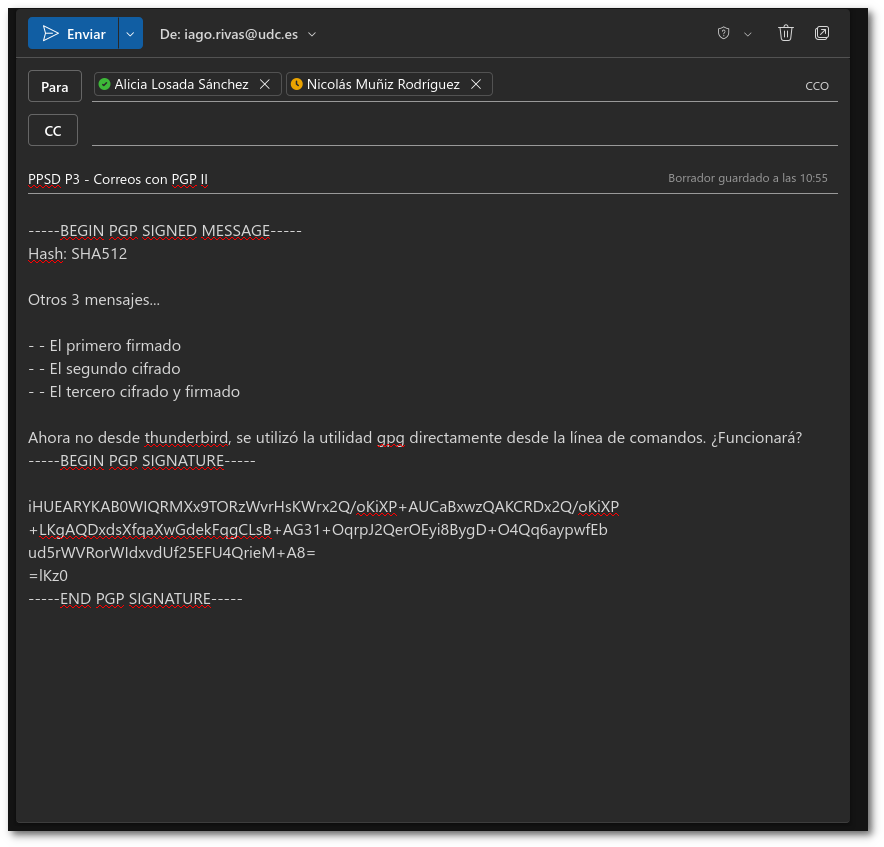
\includegraphics[width=0.9\textwidth]{outlook-firmado-sombra.png}
        \caption{Envío del mensaje firmado}
    \end{subfigure}%
    \begin{subfigure}{.5\textwidth}
        \centering
        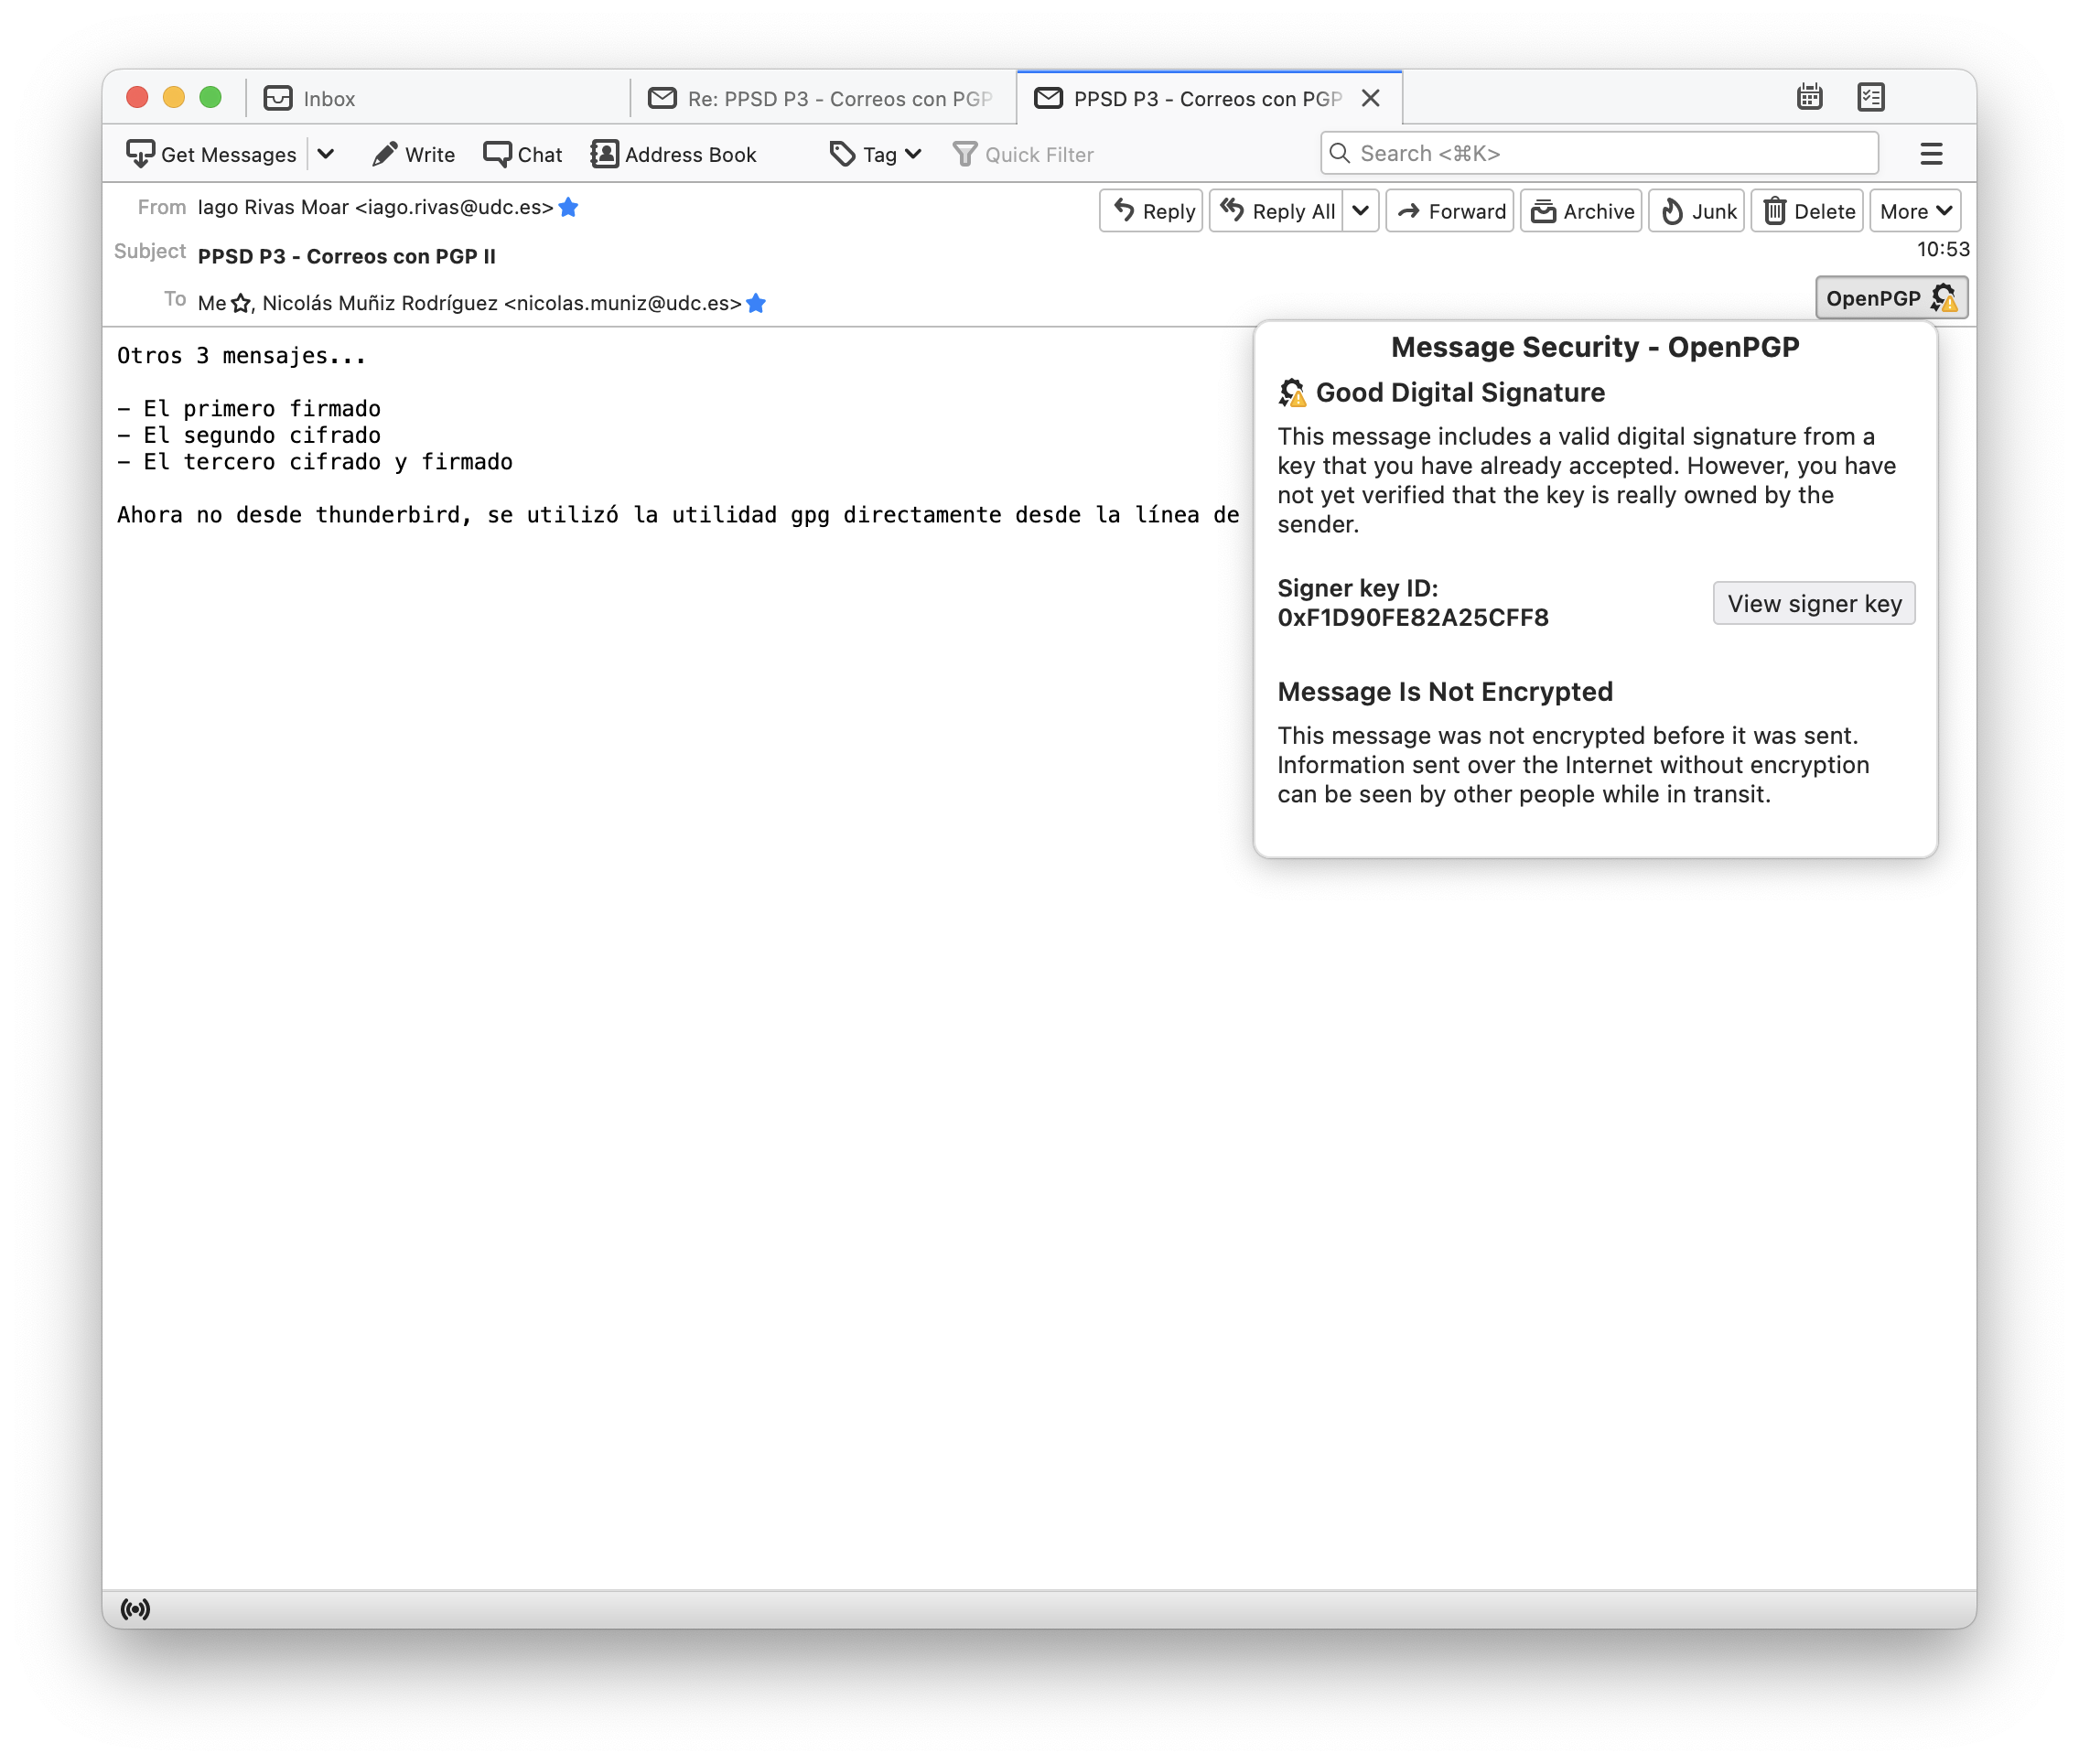
\includegraphics[width=\textwidth]{thunderbird-firmado.png}
        \caption{Recepción del mensaje firmado}
    \end{subfigure}
    \caption{Envío y recepción del mensaje firmado}
\end{figure}

\begin{tcolorbox}[
    colback=orange!5!white,
    colframe=orange!75!black,
    title=Tipos de firmas en PGP
]
Con \texttt{gpg} podemos firmar un archivo de varias formas. Esto es especialmente interesante en un caso como el anterior, cuando queremos incluír una firma en un mensaje de corre electrónico
\begin{itemize}
    \item \texttt{--sign}: Firmar el documento e incluír la firma junto al documento original. Para leer el mensaje original es necesario utilizar \texttt{gpg}.
    \item \texttt{--detatch-sign}: Firmar el documento y almacenar la firma en un documento separado.
    \item \texttt{--clearsign}: Almacenar la firma junto al documento manteniendo el contenido original legible sin \texttt{gpg}. Útil para enviar mensajes de correo electrónico.
\end{itemize}
\end{tcolorbox}

Para cifrar un correo podemos usar la opción \texttt{encrypt} indicando los recipientes del correo. En este caso no es necesario indicar la identidad, ya que al solo cifrar, nuestra clave privada no se utiliza en ningún momento. Igual que con la firma, tendremos que incluír el resultado del cifrado en el cuerpo del mensaje y si los recipientes utilizan Thunderbird verán el mensaje igual que si lo hubiéramos enviado directamente desde Thunderbird.

\begin{minted}[
    frame=single,
    framesep=8pt,
    breaklines,
    bgcolor=bgGray
]{bash}
    gpg --encrypt --armor --output correo-cif.asc -r iago.rivas@udc.es -r alicia.losada.sanchez@udc.es -r nicolas.muniz@udc.es cuerpo-correo.txt
\end{minted}

\begin{figure}[H]
    \centering
    \begin{subfigure}{.5\textwidth}
        \centering
        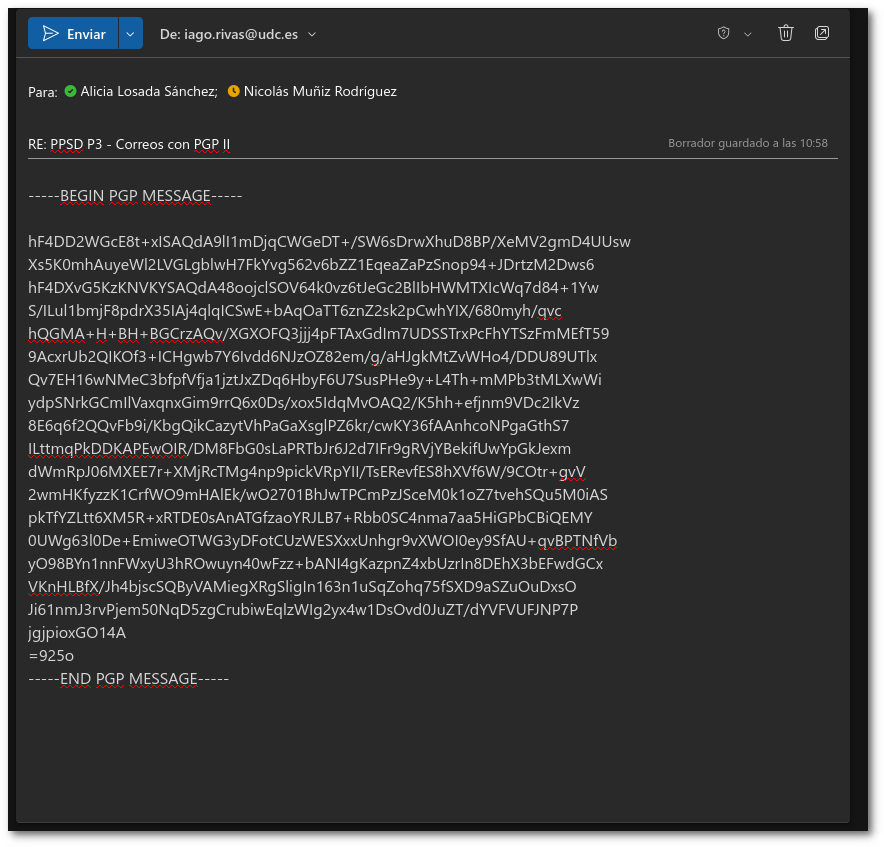
\includegraphics[width=0.9\textwidth]{outlook-cifrado-sombra.png}
        \caption{Envío del mensaje cifrado}
    \end{subfigure}%
    \begin{subfigure}{.5\textwidth}
        \centering
        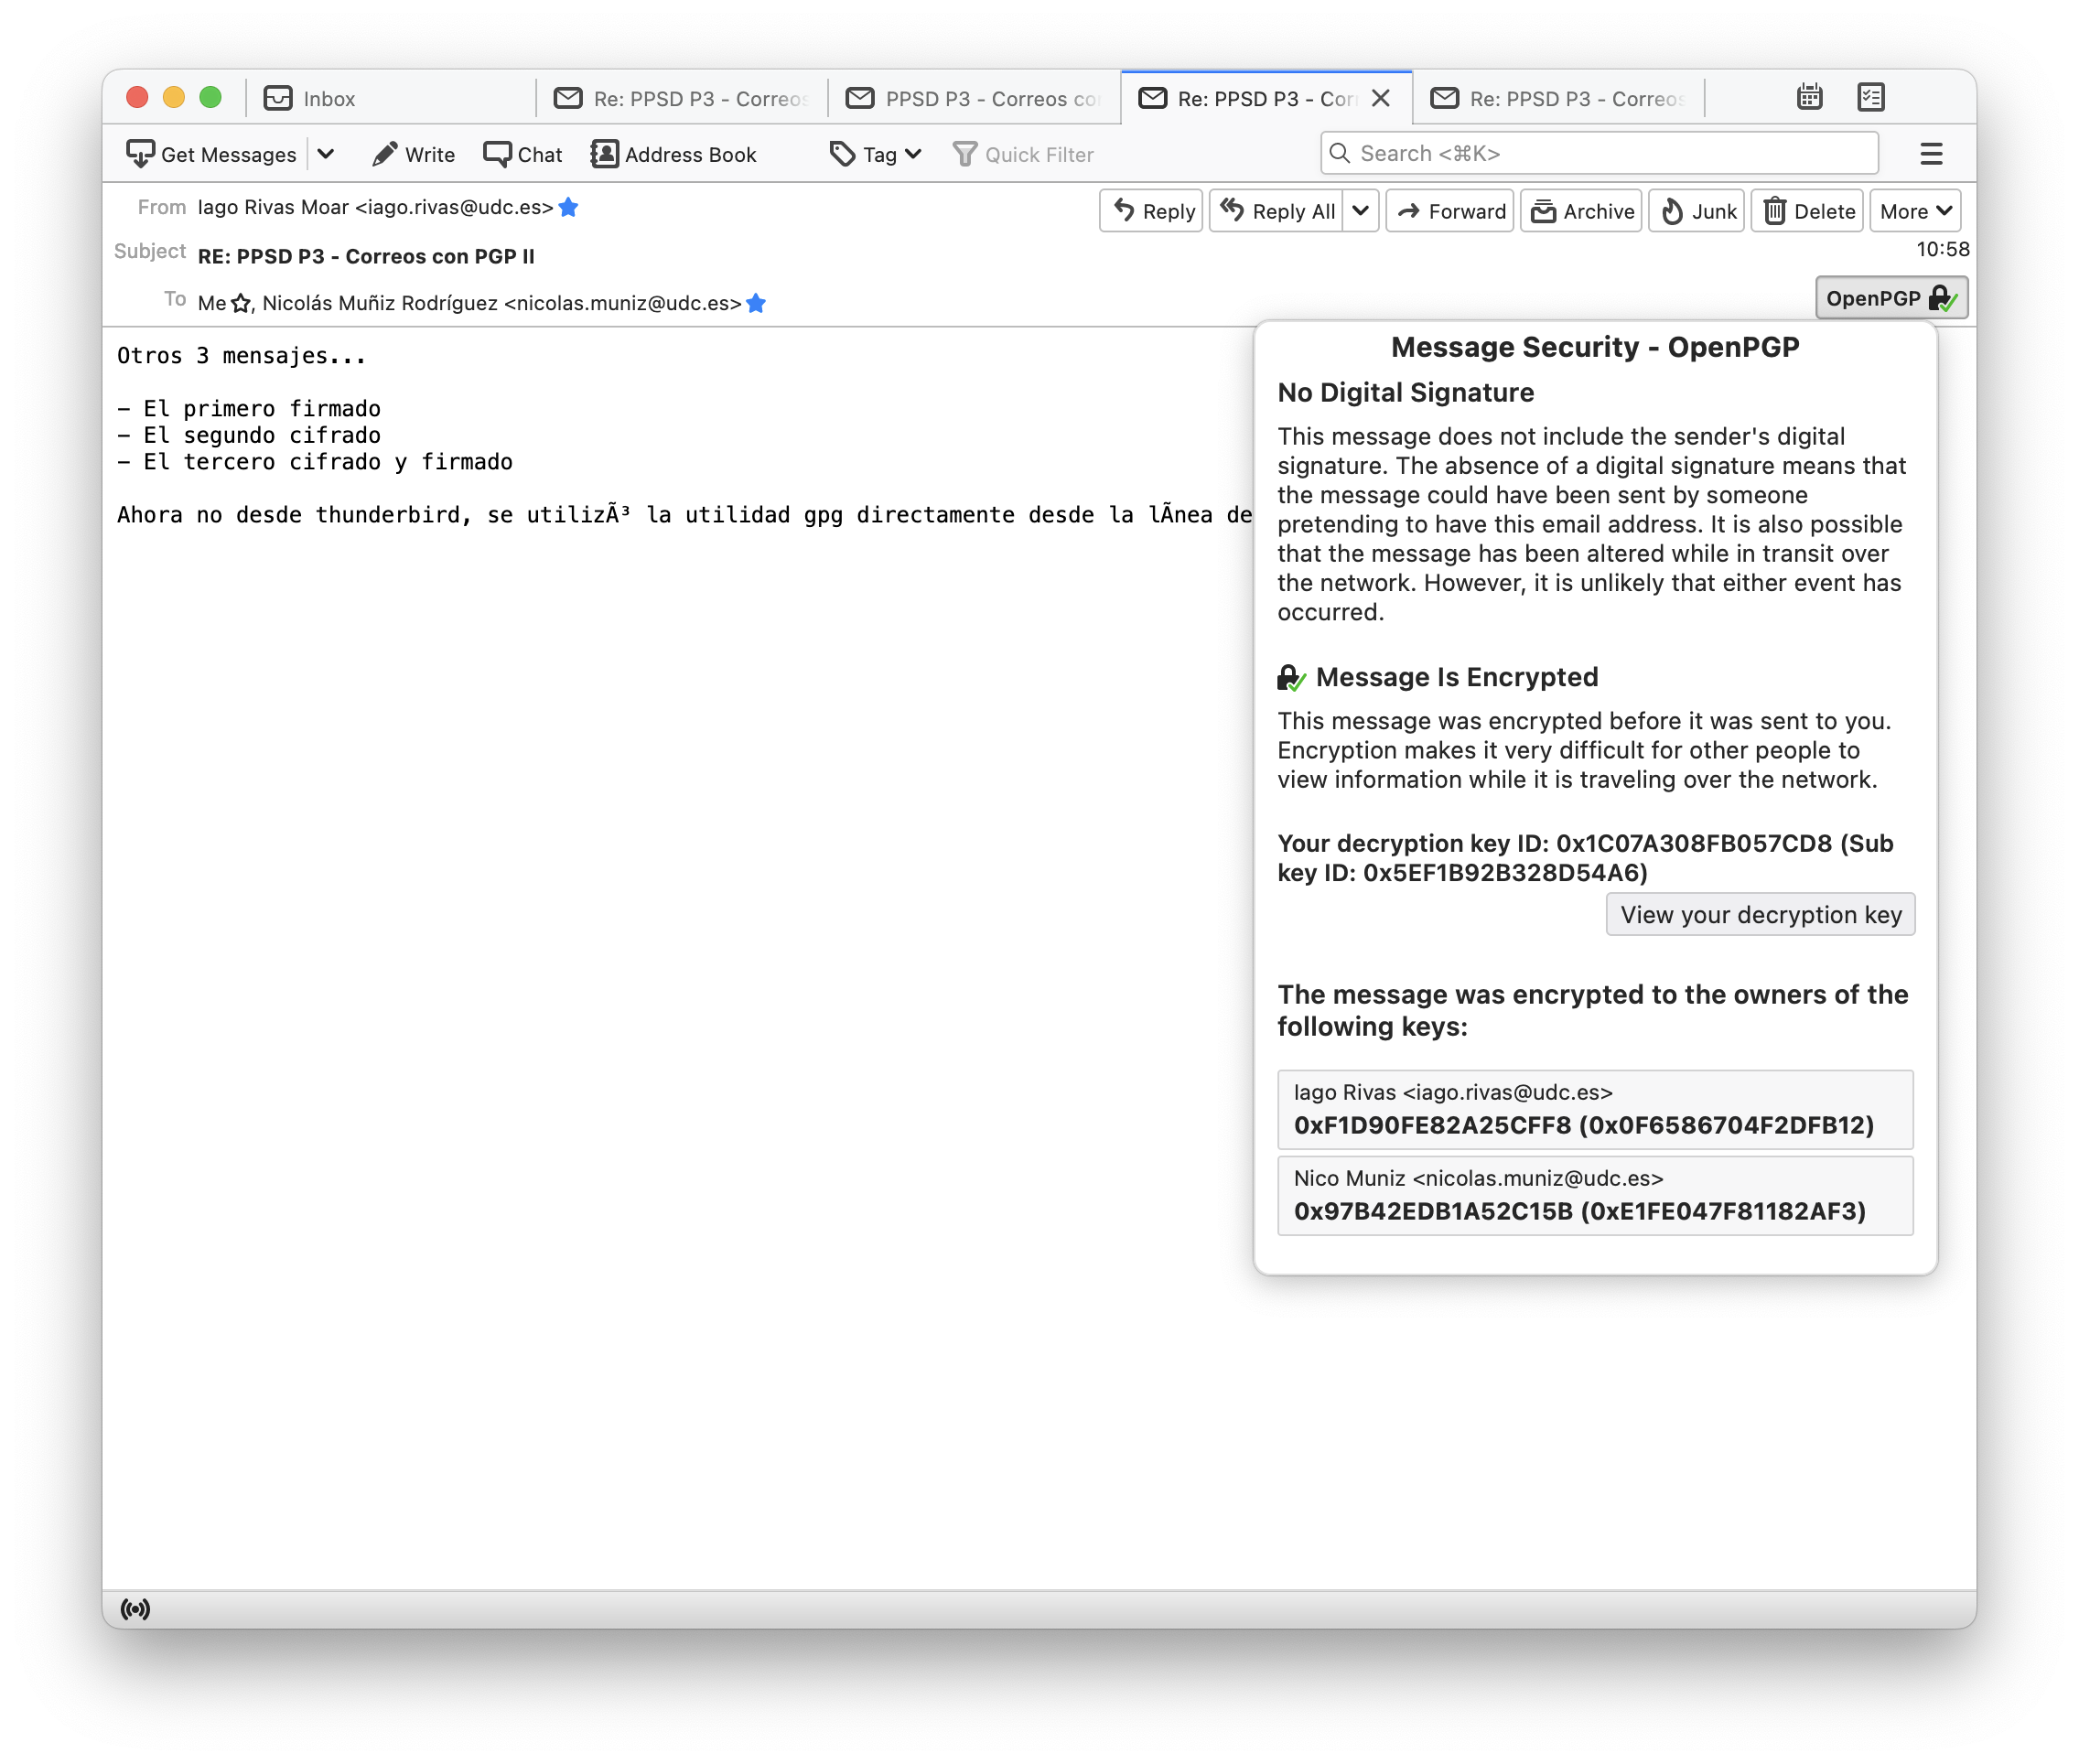
\includegraphics[width=\textwidth]{thunderbird-cifrado.png}
        \caption{Recepción del mensaje cifrado}
    \end{subfigure}
    \caption{Envío y recepción del mensaje cifrado}
\end{figure}

Por último, para firmar un correo además de cifrarlo añadiremos la opción \texttt{sign}. En este caso se vuelve a utilizar la clave privada, ya que al firmar queremos demostrar nuestra autoría del correo.

\begin{minted}[
    frame=single,
    framesep=8pt,
    breaklines,
    bgcolor=bgGray
]{bash}
    gpg --encrypt --sign --armor --output correo-cif-sig.asc -r iago.rivas@udc.es -r alicia.losada.sanchez@udc.es -r nicolas.muniz@udc.es -u iago.rivas@udc.es cuerpo-correo.txt
\end{minted}

\begin{figure}[H]
    \centering
    \begin{subfigure}{.5\textwidth}
        \centering
        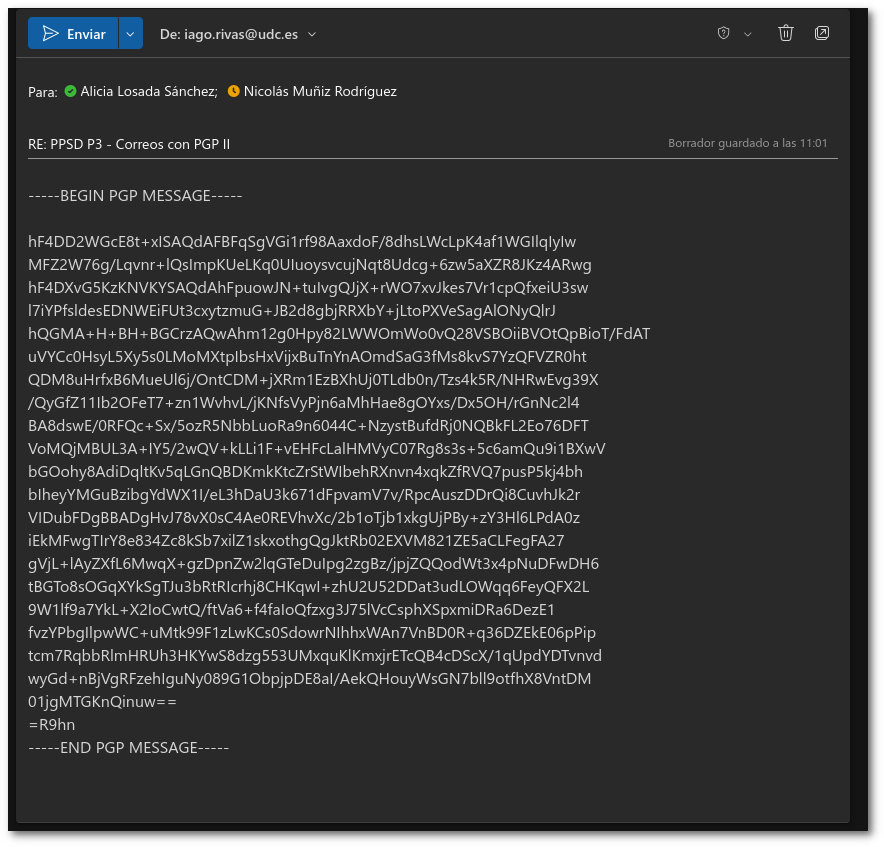
\includegraphics[width=0.9\textwidth]{outlook-firmado-cifrado-sombra.png}
        \caption{Envío del mensaje}
    \end{subfigure}%
    \begin{subfigure}{.5\textwidth}
        \centering
        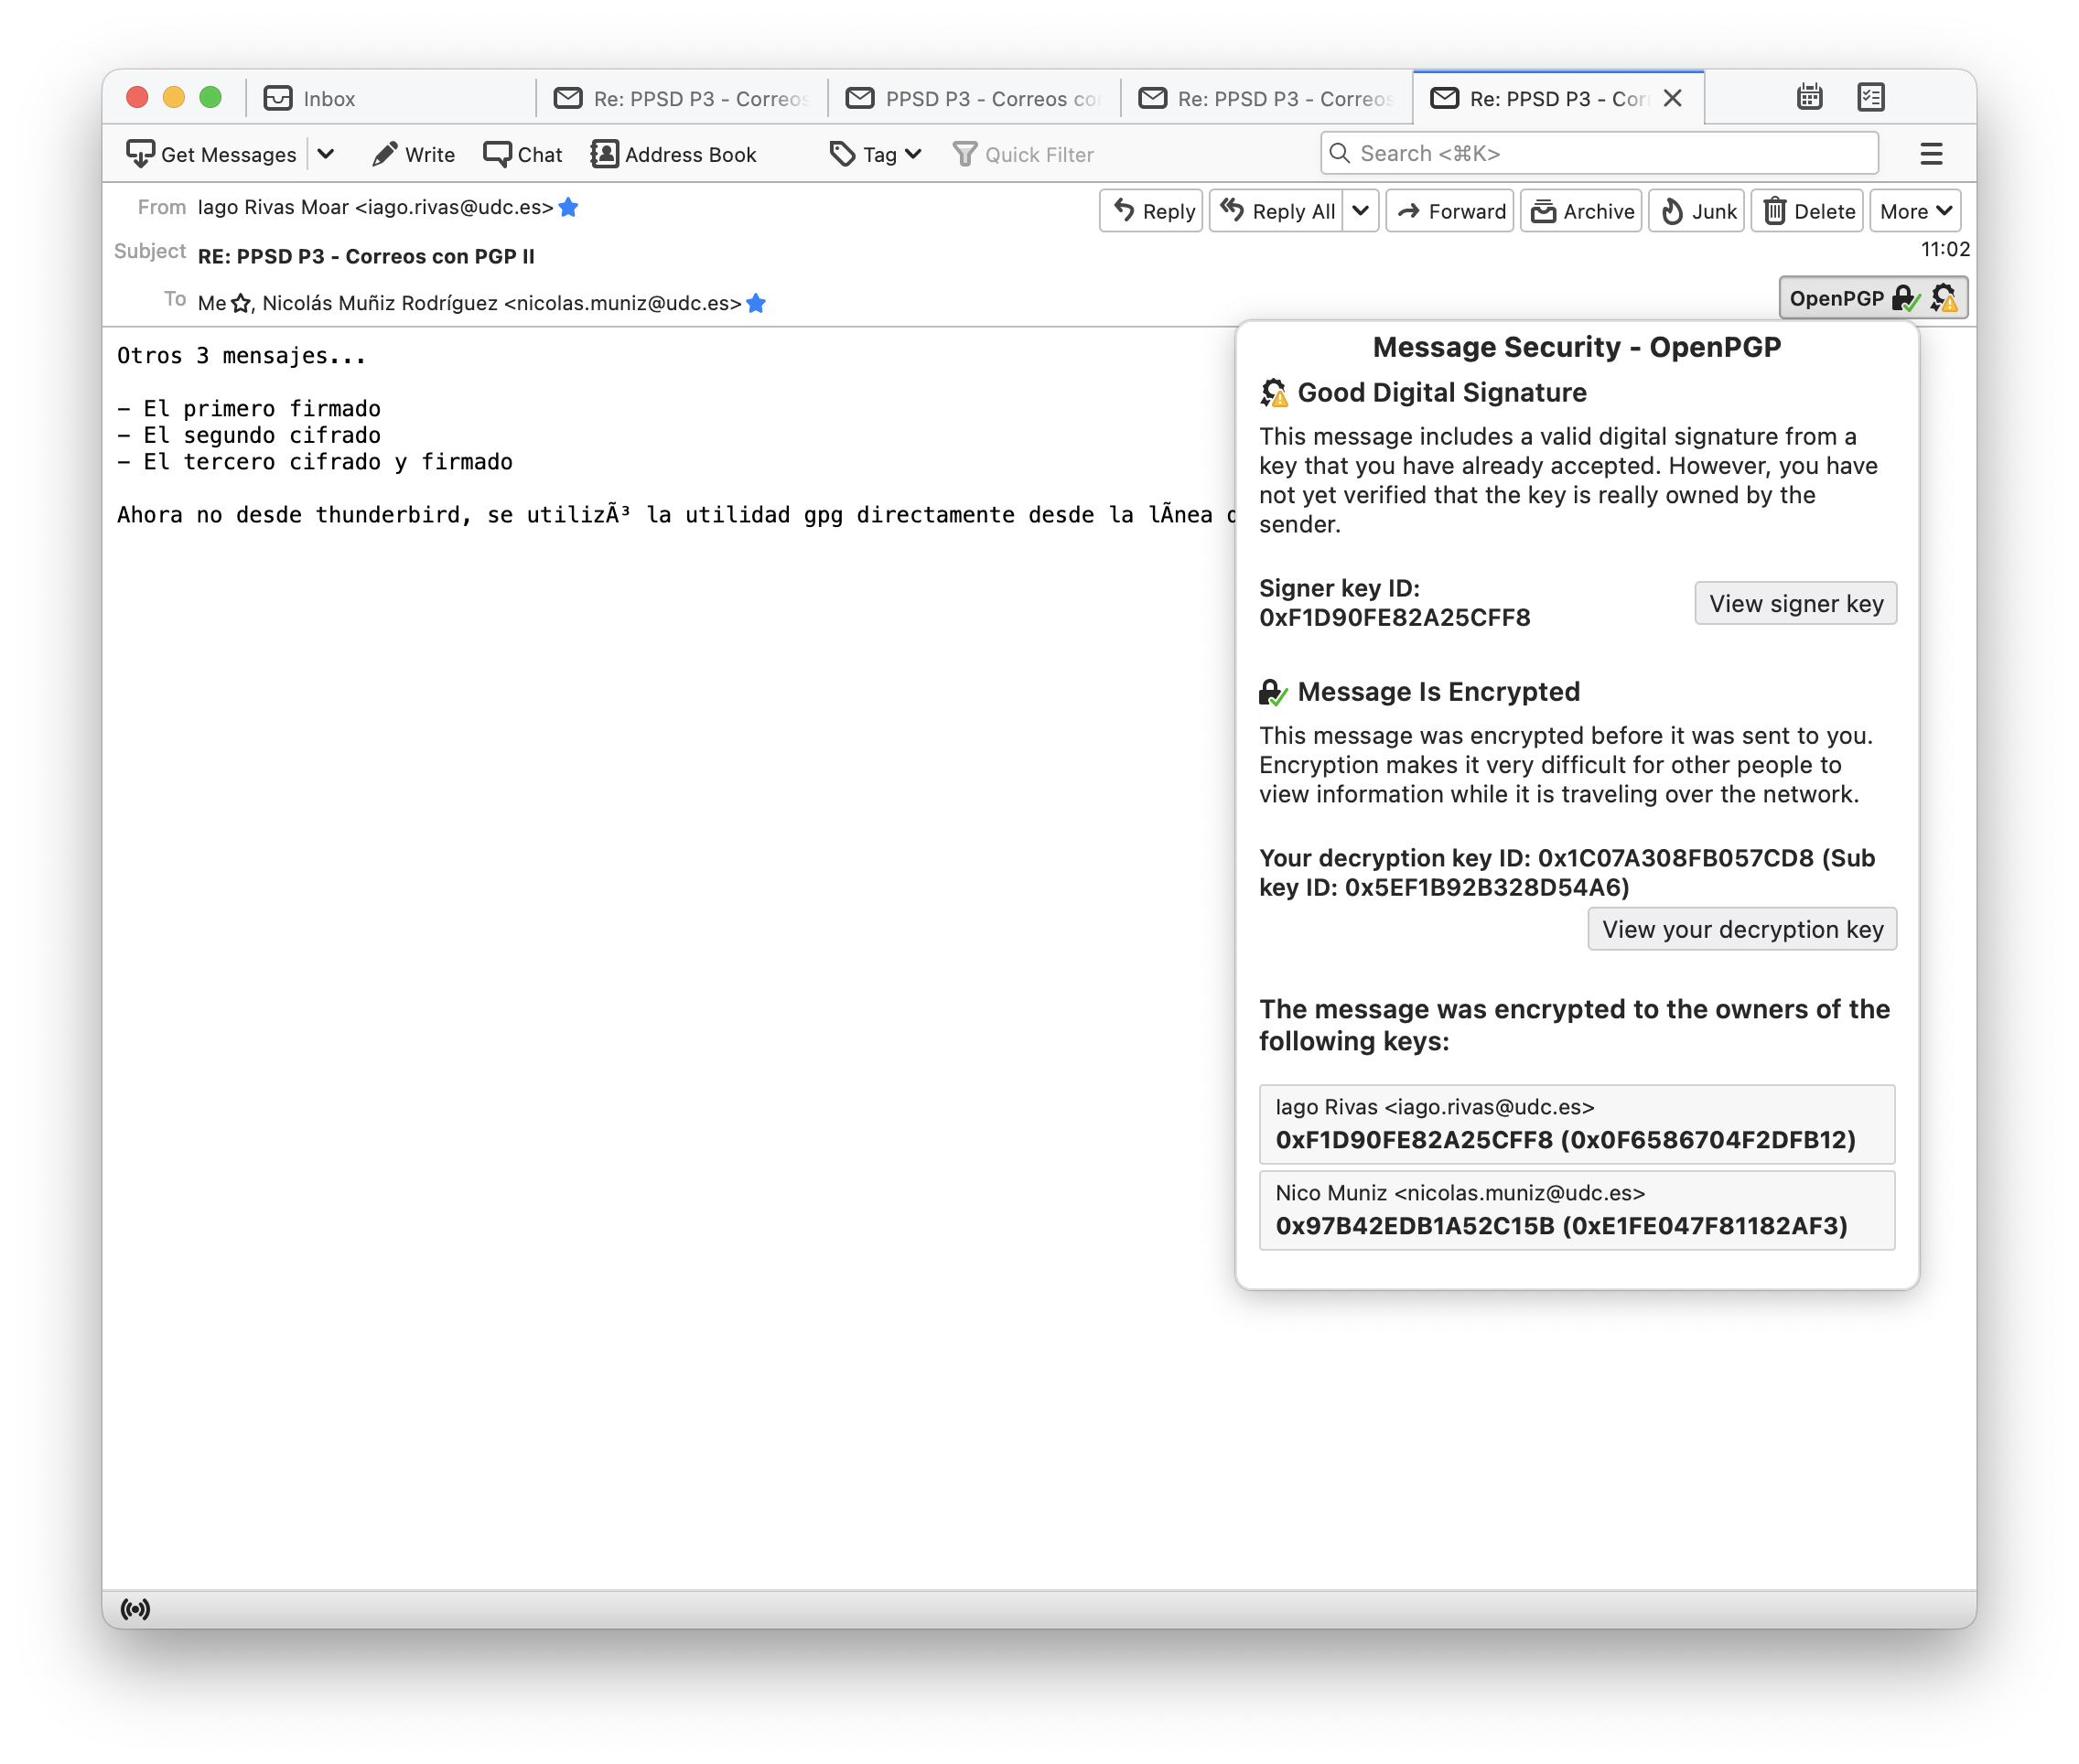
\includegraphics[width=\textwidth]{thunderbird-firmado-cifrado.png}
        \caption{Recepción del mensaje}
    \end{subfigure}
    \caption{Envío y recepción del mensaje firmado y cifrado}
\end{figure}

Aunque al enviar correos con PGP desde Thunderbird se incluyen otros archivos como la clave pública y otros metadatos, al enviar un correo con una firma o un mensaje cifrado con PGP en el cuerpo, Thunderbird lo detectará automáticamente y nos mostrará la información sobre la firma y el mensaje descifrado.

\subsubsection{Lectura de archivos con \texttt{gpg}}

Si queremos leer el contenido de los mensajes cifrados sin Thundebird podemos utilizar directamente \texttt{gpg}:

\begin{itemize}
    \item Para un mensaje firmado, podemos comprobar la firma con \\\texttt{gpg --verify firmado.asc}
    \item Para un mensaje cifrado, podemos descifrarloc on \texttt{gpg --decrypt cifrado.asc}
    \item Si el mensaje también está firmado, con el comando anterior \texttt{gpg} también mostrará si la firma es válida
\end{itemize}
